% TikZ Bar Chart for Ablation Study
% Compile with pdflatex

\documentclass{standalone}
\usepackage{pgfplots}
\usepackage{tikz}
\pgfplotsset{compat=1.17}

\begin{document}

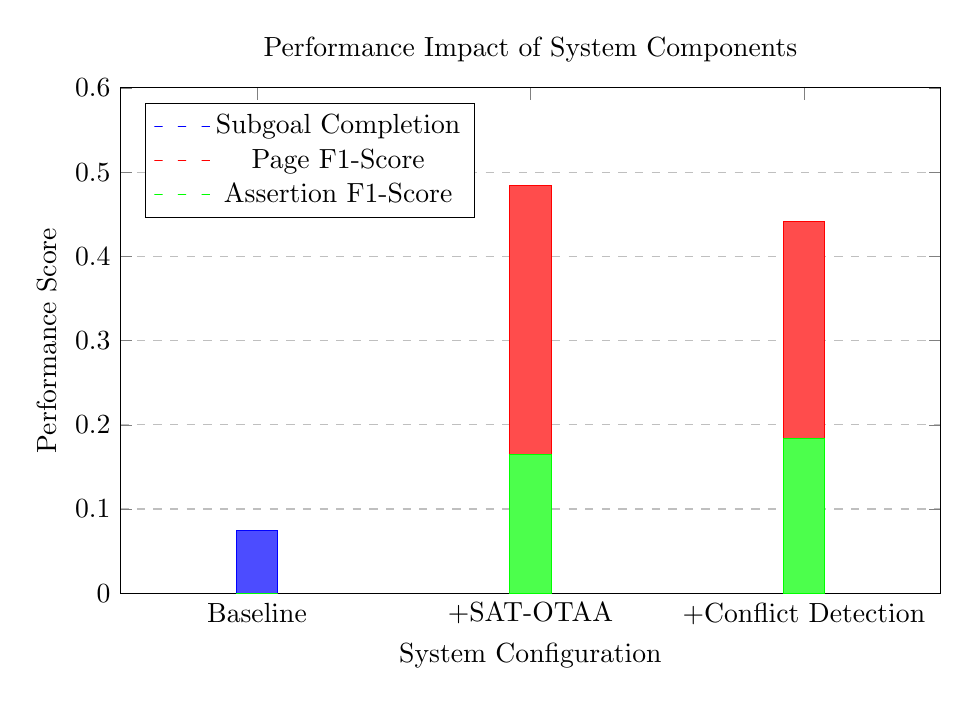
\begin{tikzpicture}
\begin{axis}[
    title={Performance Impact of System Components},
    xlabel={System Configuration},
    ylabel={Performance Score},
    xmin=-0.5, xmax=2.5,
    ymin=0, ymax=0.6,
    xtick={0,1,2},
    xticklabels={Baseline, +SAT-OTAA, +Conflict Detection},
    ytick={0,0.1,0.2,0.3,0.4,0.5,0.6},
    legend pos=north west,
    ymajorgrids=true,
    grid style=dashed,
    width=12cm,
    height=8cm,
    bar width=15pt,
]

% Subgoal Completion Rate
\addplot[
    ybar,
    fill=blue!70,
    draw=blue,
] coordinates {
    (0,0.074) (1,0.202) (2,0.227)
};

% Page F1-Score  
\addplot[
    ybar,
    fill=red!70,
    draw=red,
] coordinates {
    (0,0.000) (1,0.484) (2,0.441)
};

% Assertion F1-Score
\addplot[
    ybar,
    fill=green!70,
    draw=green,
] coordinates {
    (0,0.000) (1,0.165) (2,0.184)
};

\legend{Subgoal Completion, Page F1-Score, Assertion F1-Score}

\end{axis}
\end{tikzpicture}

\end{document}
